%%%%%%%%%%%%%%%%%%%%%%%%%%%%%%%%%%%%%%%%%%%%%%%%%%%%%%%%
\documentclass[12pt,a4paper]{article}% 文档格式
\usepackage{ctex,hyperref}% 输出汉字
\usepackage{times}% 英文使用Times New Roman
\usepackage{tcolorbox} % 用于给文字周围加框
%%%%%%%%%%%%%%%%%%%%%%%%%%%%%%%%%%%%%%%%%%%%%%%%%%%%%%%%
% 导入代码块
\usepackage{listings}
\lstdefinestyle{mystyle}{
    language=, % 设置代码的编程语言,例如Python、Bash等
    basicstyle=\small\ttfamily, % 设置代码的基本字体样式
    keywordstyle=\color{blue}, % 设置关键字的颜色
    commentstyle=\color{green!60!black}, % 设置注释的颜色
    numbers=none, % 设置行号的位置,可选值有left、right、none
    numberstyle=\tiny\color{gray}, % 设置行号的字体样式
    stepnumber=1, % 设置行号的间隔
    numbersep=1pt, % 设置行号与代码的间距
    backgroundcolor=\color{gray!10}, % 设置代码的背景颜色
    frame=single, % 设置代码框的样式,可选值有none、single、shadowbox等
    breaklines=true, % 自动换行
    showstringspaces=false, % 控制是否显示代码中的空格
    captionpos=b % 设置代码标题的位置,可选值有t、b
}

%%%%%%%%%%%%%%%%%%%%%%%%%%%%%%%%%%%%%%%%%%%%%%%%%%%%%%%%
\title{\fontsize{24pt}{24pt}\selectfont% 小四字号,1.5倍行距
	{\heiti% 黑体 
		阶段一~实验报告}\\[0.5ex] % 主标题
	{\fontsize{16pt}{24pt}\selectfont% 小三字号,1.5倍行距
		\heiti——~Gamma在液体闪烁体内的能量沉积}}% 副标题}
%%%%%%%%%%%%%%%%%%%%%%%%%%%%%%%%%%%%%%%%%%%%%%%%%%%%%%%%
\author{\fontsize{12pt}{18pt}\selectfont% 小四字号,1.5倍行距
	{\fangsong% 仿宋
		致理-数理1~~~刘苏青}\thanks{\href{mailto:liu-sq21@mails.tsinghua.edu.cn}{liu-sq21@mails.tsinghua.edu.cn}}% 标题栏脚注
        {\fangsong
        ~~~2021013371}\\
        {\fontsize{12pt}{18pt}\selectfont
        {\fangsong
        致理-物12~~~卢一鸣\thanks{\href{mailto:luym21@mails.tsinghua.edu.cn}{luym21@mails.tsinghua.edu.cn}}}
        {\fangsong
        ~~~2021013384}}\\
        {\fontsize{12pt}{18pt}\selectfont
        {\fangsong
        致理-数理1~~~马腾跃\thanks{\href{mailto:mty21@mails.tsinghua.edu.cn}{mty21@mails.tsinghua.edu.cn}}}
        {\fangsong
        ~~~2021013389}}\\
	\fontsize{10.5pt}{15.75pt}\selectfont% 五号字号,1.5倍行距
	{\fangsong% 仿宋
		2023~/~08~/~08}}
%%%%%%%%%%%%%%%%%%%%%%%%%%%%%%%%%%%%%%%%%%%%%%%%%%%%%%%%
\date{}% 日期(这里避免生成日期)
%%%%%%%%%%%%%%%%%%%%%%%%%%%%%%%%%%%%%%%%%%%%%%%%%%%%%%%%
\usepackage{amsmath,amsfonts,amssymb}% 为公式输入创造条件的宏包
%%%%%%%%%%%%%%%%%%%%%%%%%%%%%%%%%%%%%%%%%%%%%%%%%%%%%%%%
\usepackage{graphicx}% 图片插入宏包
\usepackage{animate}% gif插入宏包
\usepackage{subfigure}% 并排子图
\usepackage{float}% 浮动环境,用于调整图片位置
\usepackage[export]{adjustbox}% 防止过宽的图片
%%%%%%%%%%%%%%%%%%%%%%%%%%%%%%%%%%%%%%%%%%%%%%%%%%%%%%%%
\usepackage{bibentry}
\usepackage{natbib}% 以上2个为参考文献宏包
%%%%%%%%%%%%%%%%%%%%%%%%%%%%%%%%%%%%%%%%%%%%%%%%%%%%%%%%
\usepackage{abstract}% 两栏文档,一栏摘要及关键字宏包
\renewcommand{\abstracttextfont}{\fangsong}% 摘要内容字体为仿宋
\renewcommand{\abstractname}{\textbf{摘\quad 要}}% 更改摘要二字的样式
%%%%%%%%%%%%%%%%%%%%%%%%%%%%%%%%%%%%%%%%%%%%%%%%%%%%%%%%
\usepackage{xcolor}% 字体颜色宏包
\newcommand{\red}[1]{\textcolor[rgb]{1.00,0.00,0.00}{#1}}
\newcommand{\blue}[1]{\textcolor[rgb]{0.00,0.00,1.00}{#1}}
\newcommand{\green}[1]{\textcolor[rgb]{0.00,1.00,0.00}{#1}}
\newcommand{\darkblue}[1]
{\textcolor[rgb]{0.00,0.00,0.50}{#1}}
\newcommand{\darkgreen}[1]
{\textcolor[rgb]{0.00,0.37,0.00}{#1}}
\newcommand{\darkred}[1]{\textcolor[rgb]{0.60,0.00,0.00}{#1}}
\newcommand{\brown}[1]{\textcolor[rgb]{0.50,0.30,0.00}{#1}}
\newcommand{\purple}[1]{\textcolor[rgb]{0.50,0.00,0.50}{#1}}% 为使用方便而编辑的新指令
%%%%%%%%%%%%%%%%%%%%%%%%%%%%%%%%%%%%%%%%%%%%%%%%%%%%%%%%
\usepackage{url}% 超链接
\usepackage{bm}% 加粗部分公式
\usepackage{multirow}
\usepackage{booktabs}
\usepackage{epstopdf}
\usepackage{epsfig}
\usepackage{longtable}% 长表格
\usepackage{supertabular}% 跨页表格
\usepackage{algorithm}
\usepackage{algorithmic}
\usepackage{changepage}% 换页
%%%%%%%%%%%%%%%%%%%%%%%%%%%%%%%%%%%%%%%%%%%%%%%%%%%%%%%%
\usepackage{enumerate}% 短编号
\usepackage{caption}% 设置标题
\captionsetup[figure]{name=\fontsize{10pt}{15pt}\selectfont Figure}% 设置图片编号头
\captionsetup[table]{name=\fontsize{10pt}{15pt}\selectfont Table}% 设置表格编号头
%%%%%%%%%%%%%%%%%%%%%%%%%%%%%%%%%%%%%%%%%%%%%%%%%%%%%%%%
\usepackage{indentfirst}% 中文首行缩进
\usepackage[left=2.50cm,right=2.50cm,top=2.80cm,bottom=2.50cm]{geometry}% 页边距设置
\renewcommand{\baselinestretch}{1.5}% 定义行间距(1.5)
%%%%%%%%%%%%%%%%%%%%%%%%%%%%%%%%%%%%%%%%%%%%%%%%%%%%%%%%
\usepackage{fancyhdr} %设置全文页眉、页脚的格式
\pagestyle{fancy}
\hypersetup{colorlinks=true,linkcolor=black}% 去除引用红框,改变颜色
%%%%%%%%%%%%%%%%%%%%%%%%%%%%%%%%%%%%%%%%%%%%%%%%%%%%%%%%
\usepackage[bottom]{footmisc}
\usepackage{ulem}
\usepackage{listings}
\lstset{
  language=R,
  basicstyle=\ttfamily\footnotesize, % 设置为较小的字体大小
  keywordstyle=\bfseries\color{blue},
  commentstyle=\color{green!60!black},
  stringstyle=\color{orange},
  showstringspaces=false,
  numbers=left,
  numberstyle=\tiny,
  breaklines=true,
  frame=single,
  backgroundcolor=\color{gray!10},
  captionpos=b,
  xleftmargin=1em,
  framexleftmargin=1em,
}
\tcbuselibrary{breakable}
\begin{document}% 以下为正文内容
	\maketitle% 产生标题,没有它无法显示标题
	%%%%%%%%%%%%%%%%%%%%%%%%%%%%%%%%%%%%%%%%%%%%%%%%%%%%%%%%
	\lhead{}% 页眉左边设为空
	\chead{}% 页眉中间设为空
	\rhead{}% 页眉右边设为空
	\lfoot{}% 页脚左边设为空
	\cfoot{\thepage}% 页脚中间显示页码
	\rfoot{}% 页脚右边设为空
	%%%%%%%%%%%%%%%%%%%%%%%%%%%%%%%%%%%%%%%%%%%%%%%%%%%%%%%%
	\begin{abstract}
		\fangsong 本文首先大致概括了大作业阶段一的整体思路,然后详细阐述了git上各文件的用法,最后提出大作业实现过程中遇到的问题,并给出相应的解决方法,便于读者快速了解我们组的项目成果。
	\end{abstract}
	
	\begin{adjustwidth}{1.06cm}{1.06cm}
		\fontsize{10.5pt}{15.75pt}\selectfont{\heiti{关键词:}\fangsong{光电效应、康普顿散射、相互作用点、液体闪烁体}}\\
	\end{adjustwidth}
 
	\iffalse
	\begin{center}% 居中处理
		{\textbf{Abstract}}% 英文摘要
	\end{center}
	\begin{adjustwidth}{1.06cm}{1.06cm}% 英文摘要内容
		\hspace{1.5em}Attention!If you input "dif{}ferent", the computer will output "different", but if you input "dif\{\}ferent", the computer will output "dif{}ferent"
	\end{adjustwidth}
        \fi
	\newpage
        \tableofcontents
        \newpage


\section{整体思路}
    大作业阶段一模拟了如下过程:一个初始能量为1MeV、2MeV、5MeV或10MeV、初始顶点为(0, 0, 0)的光子,沿初始方向为x轴正方向发出,然后根据总截面通过interaction.py采样相互作用点。在相互作用点处,根据两种效应的截面大小随机选择发生哪种效应,并继续前往下一个相互作用点,直到发生光电效应为止。如果某次发生的是光电效应,则通过photoelectric.py采样电子出射角并计算电子能量;如果某次发生的是康普顿散射,则通过compton.py采样散射光子能量并计算电子能量、光子散射角和电子反冲角。
    \newpage
\section{实现方式}
    \subsection{光电效应}
    此Python脚本命名为photoelectric.py,存储在photoelectric文件夹中。你可以通过在BASH命令行中输入如下指令调用该程序,以绘制入射光子能量为ENERGY时光电效应电子出射角的分布,并将结果存储在OUTPUT-FILE-NAME.pdf中(注意,这里是对于五种原子都绘制了电子出射角分布)\par
    
    \begin{lstlisting}[style=mystyle,label=code:bash]
$ python3 ./photoelectric/photoelectric.py -e ENERGY -o OUTPUT-FILE-NAME
    \end{lstlisting}

    为避免调用单一函数时需要反复从系统文件中读取原子信息,我们将对于同一类原子(Z相同)可能调用的所有操作函数封装入了一个photoelectric类中。类中具体结构如下
    \begin{tcolorbox}[width=16cm]
        \begin{itemize}
            \item \textbf{初始化}:对应函数\_\_init\_\_。
            通过调用init\_cs(Z), init\_le\_cs(Z), init\_high(Z), init\_low(Z)四个函数将系统文件中所有有关Z原子的信息存入该类的默认信息中。这样此后对于计算插值等操作,都可以直接调用类中已有的信息,而不必重新从系统文件中进行读取。
    
            \item \textbf{截面大小插值}: 对应函数interpolation(E\_gamma, data)。
            利用numpy. searchsorted函数找到能量E\_gamma在data区间的前驱后继,以该前驱后继构成的直线在E\_gamma处取值作为插值得到的E\_gamma对应的截面大小。\textbf{注意,此函数的需要保证E\_gamma在data所包含的能量大小区间内。}
    
            \item \textbf{计算截面}:对应函数get\_single\_atom\_photoelectric\_cross\_section(E\_gamma)
            这里是根据题目要求对光子能量进行分类,最后返回“截面大小插值”的结果。(也即完成“截面大小插值”所需前提)
    
            \item \textbf{抽样光电子散射角}: 
            对应函数sampleing(E\_gamma)。直接按照题目给定的抽样方法进行了随机抽样。
        \end{itemize}
    \end{tcolorbox}
    
    除该photoelectric类外,代码中还实现了绘制入射光子能量为E\_gamma、碰撞原子核核电荷数为Z时,光电子的散射角分布图像的功能。\par
    \begin{tcolorbox}[width=16cm]
        \begin{itemize}
            \item \textbf{绘制光电子角分布曲线}:对应函数draw\_photoelectric\_theta(Z,E\_gamma)。是用于绘制关于核电荷数为Z的原子的光电子角分布曲线。 这一函数直接调用了photoelectric类中sampleing函数20000次,采样出数量足够多的光电子(在不同散射角度分布的密度不同)。此后运用高斯核密度估计得到光电子散射角分布曲线,并在[0,180]度中均匀选取2000个点,利用matplotlib.pyplot.plot函数绘制角分布曲线。   
        \end{itemize}
    \end{tcolorbox}
    
    
    \subsection{康普顿散射}
    此Python脚本命名为compton.py,使用SciPy库进行康普顿散射模拟,使用matplotlib库来可视化结果。你可以通过在BASH命令行中输入如下指令调用脚本绘制图像:    
    \begin{lstlisting}[style=mystyle,label=code:bash]
    $ python3 ./compton/compton.py -e ENERGY -o OUTPUT-FILE-NAME
    \end{lstlisting}
    
    下面逐步介绍脚本的主要组成部分和功能:
    
    \begin{tcolorbox}[width=16cm]
 
        \begin{itemize}
            \item \textbf{常量和库}:导入脚本首先导入所需的库,包括scipy.interpolate、scipy.constants、random、mat、numpy、matplotlib.pyplot、scipy.stats、os和argparse(用于接收命令行参数)。
    
            \item \textbf{命令行参数}:脚本使用argparse模块来处理命令行参数。它接受两个可选参数:-e用于指定入射光子能量,-o用于提供生成图像的输出文件名。
            
            \item \textbf{常量和单位}:脚本使用scipy.constants模块定义electron\_mass和c,以计算能量的单位为MeV。能量单位对于康普顿散射模拟是很重要的。
            
            \item \textbf{康普顿散射截面函数}:compton\_sigma\_e(E0, Z)用于计算康普顿散射截面。给定入射光子能量E0和原子序数Z,函数从预先存在的data文件中读取特定质子数单个原子在固定入射光子能量时的截面数据,若输入的入射能量E0不存在于文件中,则进行线性插值interpolate以计算所提供能量的截面。
    
            \item \textbf{散射点计算函数}:deposition\_point(E0, theta)使用给定的入射光子能量E0和散射角度$\theta$计算反冲电子的散射角度$\theta_e$。
            
            \end{itemize}
    \end{tcolorbox}  
    
    \begin{tcolorbox}[width=16cm]

        \begin{itemize}

            \item \textbf{散射光子、电子状态采样散射采样函数}:compton\_scattered\_photon\_sampling(E0)用于对散射光子进行能量采样。输入是入射光子能量E0。对于每一个输入的光子入射能量,函数会按照Klein-Nishina 公式的形式和抽样方法抽样光子出射、入射能量比例$\epsilon (\frac{E1}{E0})$和光子的散射角$\theta$,并在最后运用能量守恒,调用depoisit\_point函数计算出电子的反冲角度分布$\theta_e$,最终返回这三个数值以方便后续进行连续采样与绘图,并为相互作用连续模拟做准备。
            
            \item \textbf{散射光子能量、角度和反冲电子角度分布函数}:compton\_scattered\_photon\_ploting(E0)可视化散射光子和反冲电子的能量和角度分布。该函数调用散射采样函数迭代地对不同光子入射能量E0下散射光子的能量E、$\theta$(散射角)和$\theta_e$(反冲电子角度)进行采样(5000次),并生成了包含1000个数据点的线性等间距数组以对最后的计数数据进行高斯核密度估计,绘制出平滑美观的三分式曲线图,反映了散射光子能量、角度和反冲电子角度关于入射光子能量的分布。   
            
        \end{itemize}
        
    \end{tcolorbox}
    \subsection{相互作用点}
    此Python脚本命名为interaction.py,通过interacted(E\_gamma)函数实现了相互作用点的采样,并通过主函数中的draw\_curve()画出液闪分子和各组分原子的两种截面随能量的变化,存储在cs\_curve.pdf文件中。\par
    你可以通过在BASH命令行中输入如下指令调用程序,以生成液闪分子与各组分原子两种散射截面和入射光子能量的关系图。
    \begin{lstlisting}[style=mystyle,label=code:bash]
    $ python3 ./interaction.py 
    \end{lstlisting}
    

    该脚本具体结构如下:
    \begin{tcolorbox}[width=16cm]
        \begin{itemize}
        \item \textbf{导入数密度}:函数\texttt{extract\_density(filename)}用于从给定的gdml文件中提取元素的数密度信息,并以字典形式返回每个元素及其对应的数密度。
        \item \textbf{导入质子数}:函数\texttt{Z\_number(filename)}用于从给定的gdml文件中提取元素的质子数\texttt{Z},并以字典形式返回每个元素及其对应的质子数。
        \end{itemize}
    \end{tcolorbox}
    
    \begin{tcolorbox}[width=16cm]
        \begin{itemize}
        \item \textbf{模拟光子在液体闪烁体中的相互作用}:函数\texttt{interacted(E\_gamma)}模拟了光子在液体闪烁体中与原子发生相互作用的过程。根据输入的光子能量$E_\gamma$,返回一个布尔值来表示是进行康普顿散射还是光电效应,以及距离下一次反应的位置和与哪个原子发生的反应。
        \item \textbf{绘制两种截面随入射光子能量的变化曲线}:函数\texttt{draw\_curve()}绘制了液体闪烁体的康普顿散射截面和光电效应截面随入射光子能量的变化曲线。同时,它还返回了计算所得的液闪分子的康普顿效应截面和光电效应截面,以及入射光子能量$E_\gamma$取样点的信息。
        \end{itemize}
    \end{tcolorbox}

    \subsection{模拟液闪分子与光子的作用全过程}
    我们在main.py中实现了模拟一个光子射入液闪后与液闪分子发生相互作用全过程的功能。可以通过如下代码调用该程序,会在当前路径得到题目要求的deposit.h5文件(模拟SIMULATION-TIME个能量为ENERGY光子射入的事件)。
    \begin{lstlisting}[style=mystyle,label=code:bash]
    $ python3 ./main.py -e ENERGY -n_simulation SIMULATION-TIME
    \end{lstlisting}\par
    我们将任意时刻的光子/电子都视作对象,编写了main\_atom类。具体结构如下:
    \begin{tcolorbox}[width=16cm]
        \begin{itemize}
            \item \textbf{初始化}: 对应函数\_\_init\_\_。在类中存储了方向Direction(3维numpy array),能量Energy(float),位置Position(3维numpy array)三个变量
            
            \item \textbf{移动粒子}: 对应函数next\_atom(theta, phi, distance, new\_energy)。表示产生一个新的main\_atom类对象(意味产生一个新粒子)。
            新粒子的\textbf{随体坐标轴}是先绕\textbf{原粒子随体坐标轴}的Y轴顺时针旋转theta角,再绕\textbf{原粒子随体坐标轴}的Z轴顺时针旋转phi角。新粒子的位置是原粒子的位置沿\textbf{新粒子随体坐标轴}的Z轴正方向移动distance距离得到。新粒子的能量是new\_energy。
        \end{itemize}
    \end{tcolorbox}
    \par
    很容易发现我们需要编写一个向量绕定轴旋转的功能,我们将这个功能集成在了./tool/vector\_tool.py中。
    
    \begin{tcolorbox}[width=16cm]
        \begin{itemize}
            \item \textbf{向量绕定轴旋转}:对应代码./tool/vector\_tool.py中rotate\_vector(vector, axis, angle)函数。该函数将返回三维向量vector绕三维向量axis轴正方向,顺时针旋转angle角度后的向量
        \end{itemize}
    \end{tcolorbox}
    模拟光子入射发生的反应全过程在主函数中完成。
    \begin{center}
        \begin{tcolorbox}[width=16cm]
            \begin{itemize}
                \item \textbf{模拟所有反应过程}:在main.py的主函数中。根据调用interaction.py中的interacted(E\_gamma)函数的返回值选择此后是模拟光电效应还是康普顿散射过程。二者后续处理大致相似:采样电子散射角、能量$\rightarrow$计算光子散射角、能量(若有)$\rightarrow$利用next\_atom函数处理出新对象$\rightarrow$继续调用interacted函数采样新一轮反应(若不是光电效应)
            \end{itemize}
        \end{tcolorbox}
    \end{center}
    
\newpage
\section{小组分工}
    \begin{itemize}
        \item \textbf{刘苏青}:查找瑞利散射资料并录入其数据,编写interaction.py、interaction\_all\_extend.py程序,整理仓库,并编辑写作实验报告的主要框架及对应部分。
        \item \textbf{卢一鸣}:编写photoelectric.py、main.py、main\_all\_extend.py、main\_Rayleigh.py程序,整理仓库,并编辑写作实验报告的对应部分。
        \item \textbf{马腾跃}:编写compton.py、Rayleigh.py散射截面部分、main\_Bethe.py和Makefile文件,编写并优化画图程序analysis.py,整理仓库,并编辑写作实验报告的对应部分。
    \end{itemize}
\newpage
\section{成果复现说明}
为确保整个流程的完整性、可复现性和一次性,我们使用GNU make来组织所有的程序文件。执行特定任务需要直接在命令行中输入对应的命令,比如make all来执行所有任务,或者make pe\_theta\_1来执行单个任务(模拟光电效应)。提供的参数energy、n\_simulation可以在Makefile顶部中指定。\par
Makefile各指令具体调用方法如下:
\begin{tcolorbox}[width=16cm, breakable]
    \begin{enumerate}
        \item \textbf{make all 或 make}:
        执行所有任务,包括运行所有脚本、生成所有结果和可视化任务。
        \item \textbf{make pe\_theta\_\$(energy)}:
        运行photoelectric.py脚本模拟光电效应,生成电子出射角分布文件pe\_theta\_\$(energy).pdf。你需要在Makefile顶部更改光子能量energy。
        \item \textbf{make ce\_photo\_\$(energy)}:
        运行compton.py脚本模拟康普顿效应,生成散射光子能量分布和散射角分布,生成散射光子能量分布和散射角分布、电子出射角分布文件ce\_photo\_\$(energy).pdf。这同样需要在Makefile顶部更改光子能量energy。
        \item \textbf{make cs\_curve.pdf}:
        运行interaction.py脚本生成截面曲线pdf文档。
        \item \textbf{make Rayleigh.pdf}:
        运行Rayleigh.py脚本生成瑞利散射截面曲线pdf文档。
        \item \textbf{make deposit.h5、make deposit\_Bethe.h5和make deposit\_Rayleigh.h5}:\par
        分别运行main.py或main\_Bethe.py或main\_all\_extend模拟文件,生成模拟结果。\par
        这三个文件依次代表了"\textbf{仅考虑基本要求的模拟结果}"、"\textbf{考虑了电子的Bethe公式的模拟结果}"、"\textbf{考虑了电子的Bethe公式以及光子的瑞利散射的模拟结果}"\par
        这些需要你在Makefile顶部更改光子能量energy 和该种入射光子能量下的模拟次数n\_simulation。
        \item \textbf{make deposit(\_Bethe).html 和 make deposit(\_Bethe)\_dissymmetry.png}:
        根据模拟结果(精细考虑或不精细考虑电子与液闪分子相互作用)生成的h5文件,运行analysis.py文件,生成沉积能量的分布的可视化html和png图片。
        \item \textbf{make deposit\_all\_extend.html 和 make deposit\_all\_extend\_dissymme-try.png}:
        根据模拟结果(考虑了所有扩展结果:Bethe公式以及瑞利散射)
        生成的h5文件,运行analysis.py文件,生成沉积能量的分布的可视化html和png图片。
        \item \textbf{make clean}:
        执行清理任务,删除所有的输出文件。
    \end{enumerate}   
\end{tcolorbox}



\newpage
\section{提升部分}

    \subsection{电子沉积点的绘图形式}
    
    我们在analysis.py中实现了绘制出不同情形下电子能量沉积点的空间分布的功能。可以通过如下代码调用该程序,会在当前路径得到空间分布点文件(稍后对文件格式进行说明)。
    \begin{lstlisting}[style=mystyle,label=code:bash]
    # 沉积能量点分布
    python3 ./analysis.py -i deposit.h5
    \end{lstlisting}
    
        在绘制电子沉积点的空间分布时,我们最初选用了给出文件中要求的pdf格式。但是,如下图所示,电子沉积点的数量较多,在三维图形中,许多细节由于点过于拥挤被掩盖掉了。同时,3D散点图在平面上展示的角度是单一的,完全无法看出空间分布的规律。
  
        \begin{figure}[hb]
            \centering
            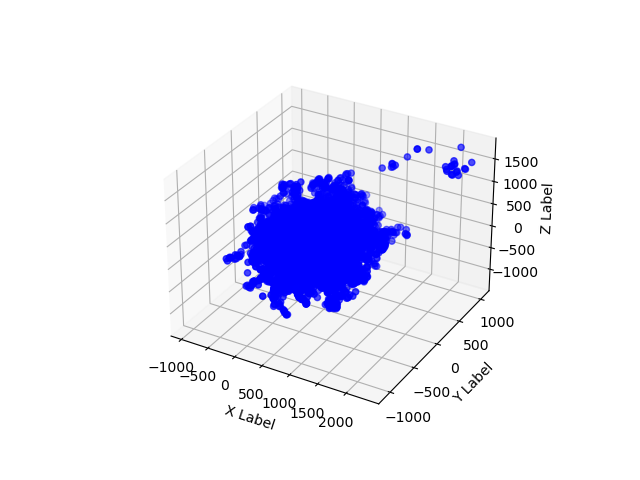
\includegraphics[width=0.6\textwidth]{raw_analysis.png}
            \caption{效果很不好的三维散点图}
            \label{fig:raw_analysis}
        \end{figure}

        在查阅相关资料后,我们选择了创建html格式的可交互式三维散点图,并调整了散点的不透明度为0.2,以达到较好的观察与呈现效果。
        但是,从采样的过程中我们可以得知,三点关于x轴应当是旋转对称分布的。也就是说,沿x轴的剖面上的信息可能会更有价值。为了更直观、更准确地表现出相互作用点的分布密度,我们采用了二维分层设色“等高线”图来展现x-z平面上的信息。图中,像素的颜色代表了这一区域相互作用点分布的密度(归一化)。这样,结合三维可交互式散点图与二维密度分布图,我们能对相互作用点的分布有着更为清晰的认知。为了使边缘清晰、分布直观,我们对相互作用点的分布再一次采用了高斯核密度估计。
        
        \begin{figure}[h]
            \centering
            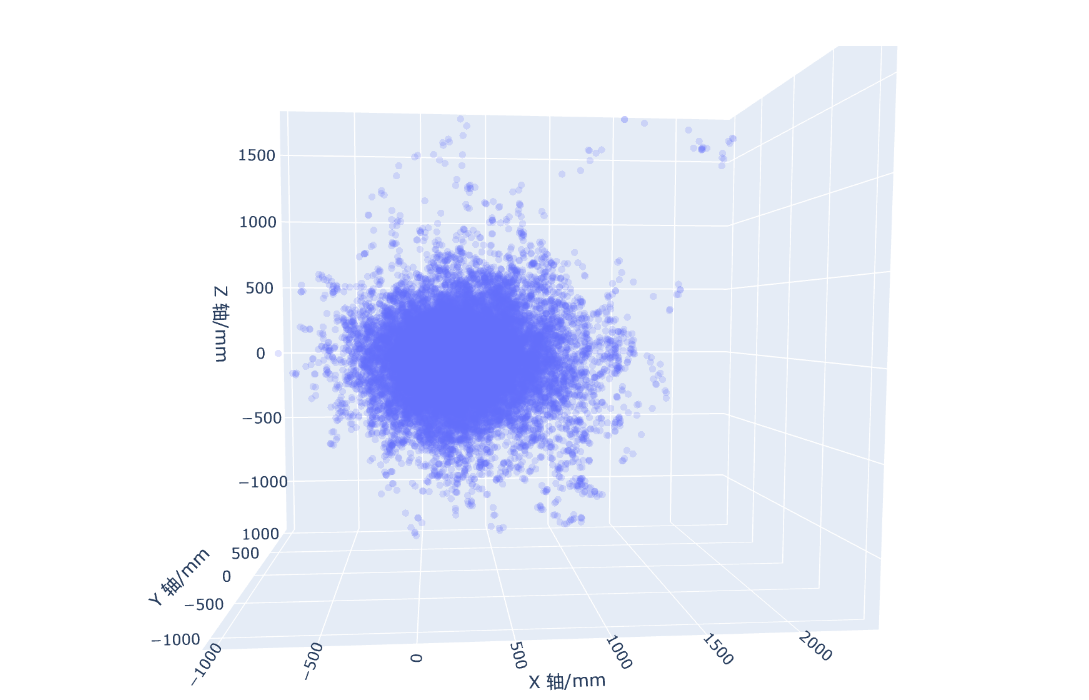
\includegraphics[width=0.6\textwidth]{deposit.png}
            \caption{可交互的三维散点图演示(入射光子能量:1MeV)}
            \label{fig:deposit_gif}
        \end{figure}
        \begin{figure}[h]
            \centering
            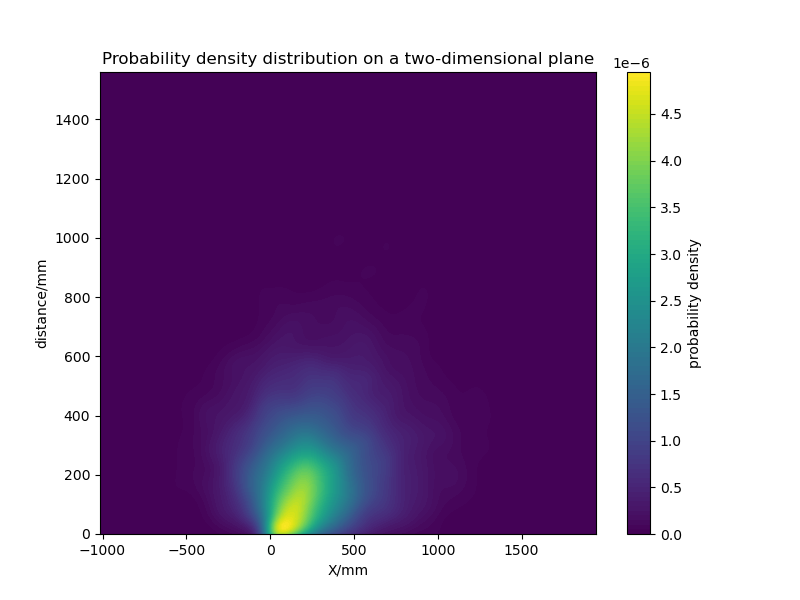
\includegraphics[width=0.6\textwidth]{deposit_dissymmetry.png}
            \caption{二维消对称电子沉积点分布图(入射光子能量:1MeV)}
            \label{fig:deposit_dissymmetry}
        \end{figure}
    \subsection{使用 Bethe 公式精细考虑电子在液闪中的能量沉积}
        
    我们在analysis.py中实现了绘制出不同情形下电子能量沉积点的空间分布的功能。通过如下代码调用该程序,会在当前路径得到精细考虑电子与液闪分子相互作用的空间分布点文件。
    \begin{lstlisting}[style=mystyle,label=code:bash]
    # 考虑Bethe公式的沉积能量点分布
    python3 ./analysis.py -i deposit_Bethe.h5
    \end{lstlisting}
    
        不同出射能量的电子,在液闪分子中的运动距离显然应该不同。在上面的部分中将其均视为运动2mm,是非常粗糙的一种估计。因此,需要引入Bethe公式,定量考虑运动电子在液闪分子中的电离和辐射能损。
        
        \begin{itemize}
            \item 电离能损(低能为主):
                {\scriptsize
                    \begin{equation*}
                    \left(-\frac{d E}{dx}\right)_{ion} =
                    \left(\frac{1}{4\pi\epsilon_0}\right)^2 \cdot \frac{2\pi e^4 N
                    Z}{m_e v^2} \times \left[\ln \frac{m_e v^2 E}{2I^2 (1 - \beta^2)
                    }- (\ln 2) (2 \sqrt{1 - \beta^2} - 1 + \beta^2) + (1 - \beta^2) +
                    \frac{1}{8}(1 - \sqrt{1-\beta^2})^2\right]
                    \end{equation*}
                }
            \item 辐射能损(高能为主):
                \begin{equation*}
                \left(-\frac{dE}{dx}\right)_{rad} = \left(\frac{1}{4\pi
                \epsilon_0}\right)^2 \cdot \frac{NEZ(Z+1)e^4}{137 m_e c^4} \cdot
                \left(4\ln \frac{2E}{m_e c^2} - \frac{4}{3}\right)
                \end{equation*}
        \end{itemize}
        
        由于低能和高能的界限并不清晰,在程序的每一步中我们都考虑了两种能损。要注意的是,为了避免歧义,我们在公式中全部使用了国际单位制,并在输出运动距离时重新将米转换为了毫米。程序的具体实现方式如下:
        
        \begin{enumerate}
            \item 将main.py中的“2”更换为传入电子出射能量的函数Bethe\_x(elec\_energy)
            \item 实现函数Bethe\_x(E):
                \begin{itemize}
                    \item 数值准备:
                    对于公式中的N,即靶粒子数密度,我们采用了所有原子的数密度之和,这样才能够更合理地反映电子与所有粒子的相互作用;对于公式中的Z,即质子数,我们假设每个步长中选取唯一的Z值,并按照各种原子在液闪物质中的数密度作为权重进行随机选择,以较好地模拟出电子与各元素原子之间的相互作用过程。综合权衡精度与计算速度,我们暂时选取一步的步长为0.001mm。
                    \item calculate\_ion\_loss(E, step, Z): 这个函数用于计算电离损失,参数E代表电子能量,step是每一步迭代的间距,Z是目标原子的原子序数。在这个函数中,首先计算洛伦兹因子($\gamma$),确定电子的速度(v),然后利用Bethe公式(尝射能量损失公式)计算每一步的能量损失。
                    \item calculate\_rad\_loss(E, step, Z): 这个函数用于计算辐射损失,参数与上述相同。这个函数主要应用于高能量电子的情况,使用了Bethe-Heitler公式。
                    \item 在主循环部分,程序首先确定了本次迭代过程中电子碰撞的原子种类(chosen\_element)。然后,计算相应的能量损失,并从电子总能量中减去这部分能量。同时,更新电子穿过的距离。循环会持续进行直到电子的能量低于特定阈值(如$10^{-30}$J)。
                \end{itemize}
        \end{enumerate}
        
        在精细考虑电子在液闪分子中的沉积过程之后,我们又进行了图像的绘制。为方便对比,这里只展示消除对称性之后的剖面图像:
        
        \begin{figure}[hb]
            \centering
            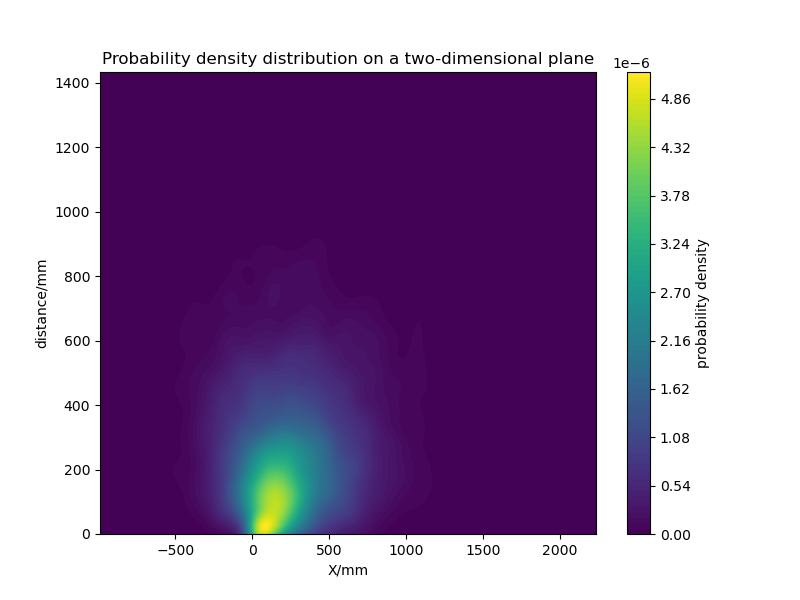
\includegraphics[width=0.6\textwidth]{deposit_Bethe_dissymmetry.png}
            \caption{精细考虑后的消对称电子沉积点分布图(入射光子能量:1MeV)}
            \label{fig:deposit_dissymmetry_Bethe}
        \end{figure}
        
        从图4中能够直观的看出,与图3相比,电子沉积点向z(y)方向的扩散距离比不考虑该效应时比较接近。并且注意到,在密度较高的区域,沉积点分布更为集中。这与h5文件中存储的数据相符合,即电子能量较高时电子的运动距离明显大于2mm,而在电子能量降低为0.01MeV或更低之后运动距离便远远小于2mm。

    \subsection{一个根据任一概率密度函数进行抽样的方法}
    在考虑瑞利散射的问题中,需要解决如何根据任一个已知的概率密度函数进行抽样的问题,我们将方法列写如下。\par
    记随机变量x服从分布函数为F(x),概率密度函数为P(x),满足$\frac{\mathrm dF}{\mathrm dx}=P$。考虑这个函数分布在[$x_{min},x_{max}$]中,选取若干个散点满足
    $$
    x_1=x_{min}<x_2<\dots<x_{N-1}<x_{N}=x_{max}
    $$\par
    此后我们令$\xi_i = F(x_i)$。根据概率论知识,若我们能够知道函数$F^{-1}(\xi_i)= x_i$在任意$\xi$处的取值,我们就可以通过向$F^{-1}$中填入一个均匀分布$\xi$,得到一个满足分布函数为$F(x)$的随机变量$x$\par
    于是要解决的问题就是如何得到任意$\xi$处,$F^{-1}(\xi)$的值。一个显然的想法是线性插值,但这会造成较大的误差。比较好的做法是使用rational interpolation。\par
    对于任一个$\xi$,显然我们能找到唯一的一个$i$,满足$\xi_i\leq \xi < \xi_{i+1}$。我们进行如下拟合。
    $$
    F^{-1}(\xi) = x_i + \frac{1+a_i+b_i}{1+a_i\eta+b_i\eta^2}(x_{i+1}-x_i)
    $$\par
    其中$\eta \equiv \frac{\xi - \xi_{i}}{\xi_{i+1}-\xi_{i}}$。根据一系列关于$a_i,b_i$的边界条件限制,可以推导出他们的取值如下\par
    \begin{align}
    b_i &= 1 - \left(\frac{\xi_{i+1}-\xi_{i}}{x_{i+1}-x_{i}}\right)^2\frac{1}{p(x_{i+1})p(x_i)} \\
    a_i &= \frac{\xi_{i+1}-\xi_{i}}{x_{i+1}-x_{i}}\frac{1}{p(x_i)}-b_i-1
    \end{align}\par
    其中$p(x_i)$是x服从的概率密度函数在$x_i$处的取值。则进一步我们可以直接推出对于均匀分布抽样得到的$\xi$,其对应的$x$为\par
    $$
    x = x_i + \frac{(1+a_i+b_i)\eta}{1+ a_i\eta + b_i\eta^2}(x_{i+1}-x_i)
    $$\par
    这个算法名叫RITA (Rational Inverse Transform with Aliasing) algorithm。
    \subsection{在模拟过程中考虑瑞利散射\cite{penelope2006workshop} } 
    \subsubsection{散射截面的计算}
        此Python脚本命名为Rayleigh.py,使用SciPy库进行瑞利散射模拟,使用matplotlib库来可视化结果。你可以通过在BASH命令行中输入如下指令调用脚本绘制瑞利散射截面图像并保存为Rayleigh.pdf:    
    \begin{lstlisting}[style=mystyle,label=code:bash]
    $ python3 ./Rayleigh/Rayleigh.py E
    \end{lstlisting}
    
        瑞利散射的单个原子总散射截面计算公式\cite{penelope2006workshop}为:
        $$\sigma_{Ra} = \int \frac{\mathrm d\sigma_{Ra}}{\mathrm d\Omega} \mathrm d\Omega = \pi r_e^2 \int \left(1 + \cos^2 \theta\right) \left[F(x, Z)\right]^2 \, \mathrm  d(\cos \theta)$$

        其中,$r_e$为电子经典半径,$F(x, Z)$称为原子散射因子,为一无量纲量。$x = \frac{\sin\left(\frac{\theta}{2}\right)}{\lambda}$,其中,$\lambda$为入射光的波长,单位为\, \text{\AA}。对不同质子数Z的原子,$F$与$x$的关系表见data/Rayleigh/F-x-\{Z\}.dat\cite{hubbell1975atomic}。对于不在表中的数据,我们采用线性插值来进行计算(越界则1111111111)。具体实现细节与2.2康普顿散射部分非常相似,这里就不再赘述。
        
        对于积分的计算,我们采用数值求积法,将-1到1划分为100个区间,分别近似求得积分函数大小后再乘以区间宽度0.02,并相加得到近似计算结果。

        \subsubsection{散射角采样}
        光子散射角$\theta$的余弦值$\cos\theta$满足如下概率密度函数\par
        $$
        p_{Ra}(\cos\theta) = \frac{1+\cos^2\theta}{2}[F(x,Z)]^2
        $$\par
        记$\kappa \equiv \frac{E_c}{m_ec^2}$,则$x$有上界
        $$
        x_{max} = 20.6074 \times 2\kappa
        $$\par
        我们记$\pi(x^2) \equiv [F(x,Z)]^2$,则$x^2\equiv t$的取值是$[0,x_{max}^2]$。可以将$\pi(t)$视作一个关于$t$的概率密度函数(需要进行归一化)。因此,抽样过程如下\par
        \begin{itemize}
            \item 使用RITA algorithm,根据$\pi(t)$抽样一个随机数$t\in[0, x_{max}^2]$

            \item 令
            $$
            \cos\theta = 1 - \frac{1}{2}\frac{t}{(20.6074\kappa)^2}
            $$
            \item 生成一个[0,1]均匀的随机数$\xi$
            \item 如果$\xi > \frac{1+\cos^2\theta}{2}$,返回第一步
            \item 否则,就抽样出了一个合法的$\cos\theta$
        \end{itemize}

        \subsubsection{加入主程序}
        事实上非常简单,但为了便于助教对比,我们重新编写了main\_all\_extend.py以及interaction\_all\_extend.py代码。\par
        在interacted函数中,我们将瑞利散射的截面也计入了总截面中,并根据三类截面大小抽样得到本次相互作用的原子及相互作用方式。\par
        在主函数中,我们新增了一项判断瑞利散射的过程。在这个过程中实际上只需要将光子转向,这可以通过2.4中提到的main\_atom类轻松实现

        \subsubsection{复现方式}
        我们也将这一部分加入了Makefile。可以通过make指令来绘制各原子和液闪分子瑞利散射截面和入射光子能量的关系图,以及进行考虑瑞利散射的全相互作用过程模拟。具体内容见4 成果复现说明部分。

        \subsubsection{模拟结果呈现}
        在考虑瑞利散射并精细考虑电子与液闪分子的相互作用之后,我们又进行了图像的绘制。为方便对比,这里只展示消除对称性之后的剖面图像:
        
        \begin{figure}[hb]
            \centering
            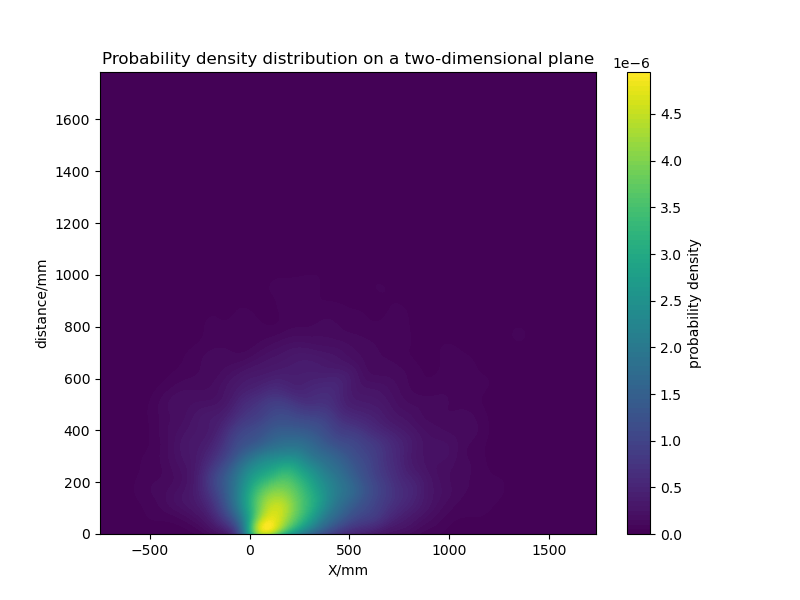
\includegraphics[width=0.6\textwidth]{deposit_all_extend_dissymmetry.png}
            \caption{精细考虑并加入瑞利散射后的消对称电子沉积点分布图(入射光子能量:1MeV)}
            \label{fig:deposit_all_extend_dissymmetry}
        \end{figure}
        
        从图5中能够直观的看出,与图4相比,电子向y、z方向的扩散距离比不考虑瑞利散射时更长一些,集中区域较分散一些。这与散射起到的作用相符合,即光子能量较低时光子的散射角度比较大,导致光子到达的空间范围比较大。事实上,这一部分的随机性很大,我们多次运行了程序,发现可扩散到的范围非常大。        
\bibliographystyle{plain}  % 指定引用样式(可以根据需要更改)
\bibliography{stage1.bib}      % 指定 BibTeX 文件(去掉扩展名)    
\end{document}
